% Capítulo 3 — Parte 1: Diseño del sistema (diseño_conceptual.tex)
\section{Diseño Conceptual}
\label{sec:prop-intro}

Este capítulo presenta el diseño y el desarrollo del sistema propuesto: una plataforma web conectada a un servicio de agentes de inteligencia artificial que permite diseñar, calcular con valores definidos, simular en \texttt{ngspice}, analizar y documentar circuitos analógicos de corriente alterna y corriente directa (CA/CD) a partir de una descripción en lenguaje natural.

El funcionamiento general del sistema se divide en cuatro fases: describir, diseñar, verificar y entregar. En la primera fase (\textit{describir}), el usuario pide su circuito con sus propias palabras desde la interfaz web. En la segunda fase (\textit{diseñar}), los agentes de inteligencia artificial interpretan el pedido, identifican los parámetros eléctricos y calculan los componentes necesarios. En la tercera fase (\textit{verificar}), el sistema arma el circuito con valores definidos, lo simula en \texttt{ngspice} y revisa si cumple la meta; cuando hay alguna desviación, ajusta los valores y vuelve a simular hasta corregirla. Por último, en la cuarta fase (\textit{entregar}), el usuario recibe el circuito validado con su esquema, sus gráficas, el código SPICE, la lista de materiales y la explicación del diseño, como se muestra en la figura~\ref{fig:diseno-conceptual-fases}.

\begin{figure}[H]
    \centering
    \makebox[\textwidth][c]{%
        % Preferir versión vectorial SVG: ../src/diagrams/diseno_conceptual_fases.svg
        \hspace*{-0.5cm}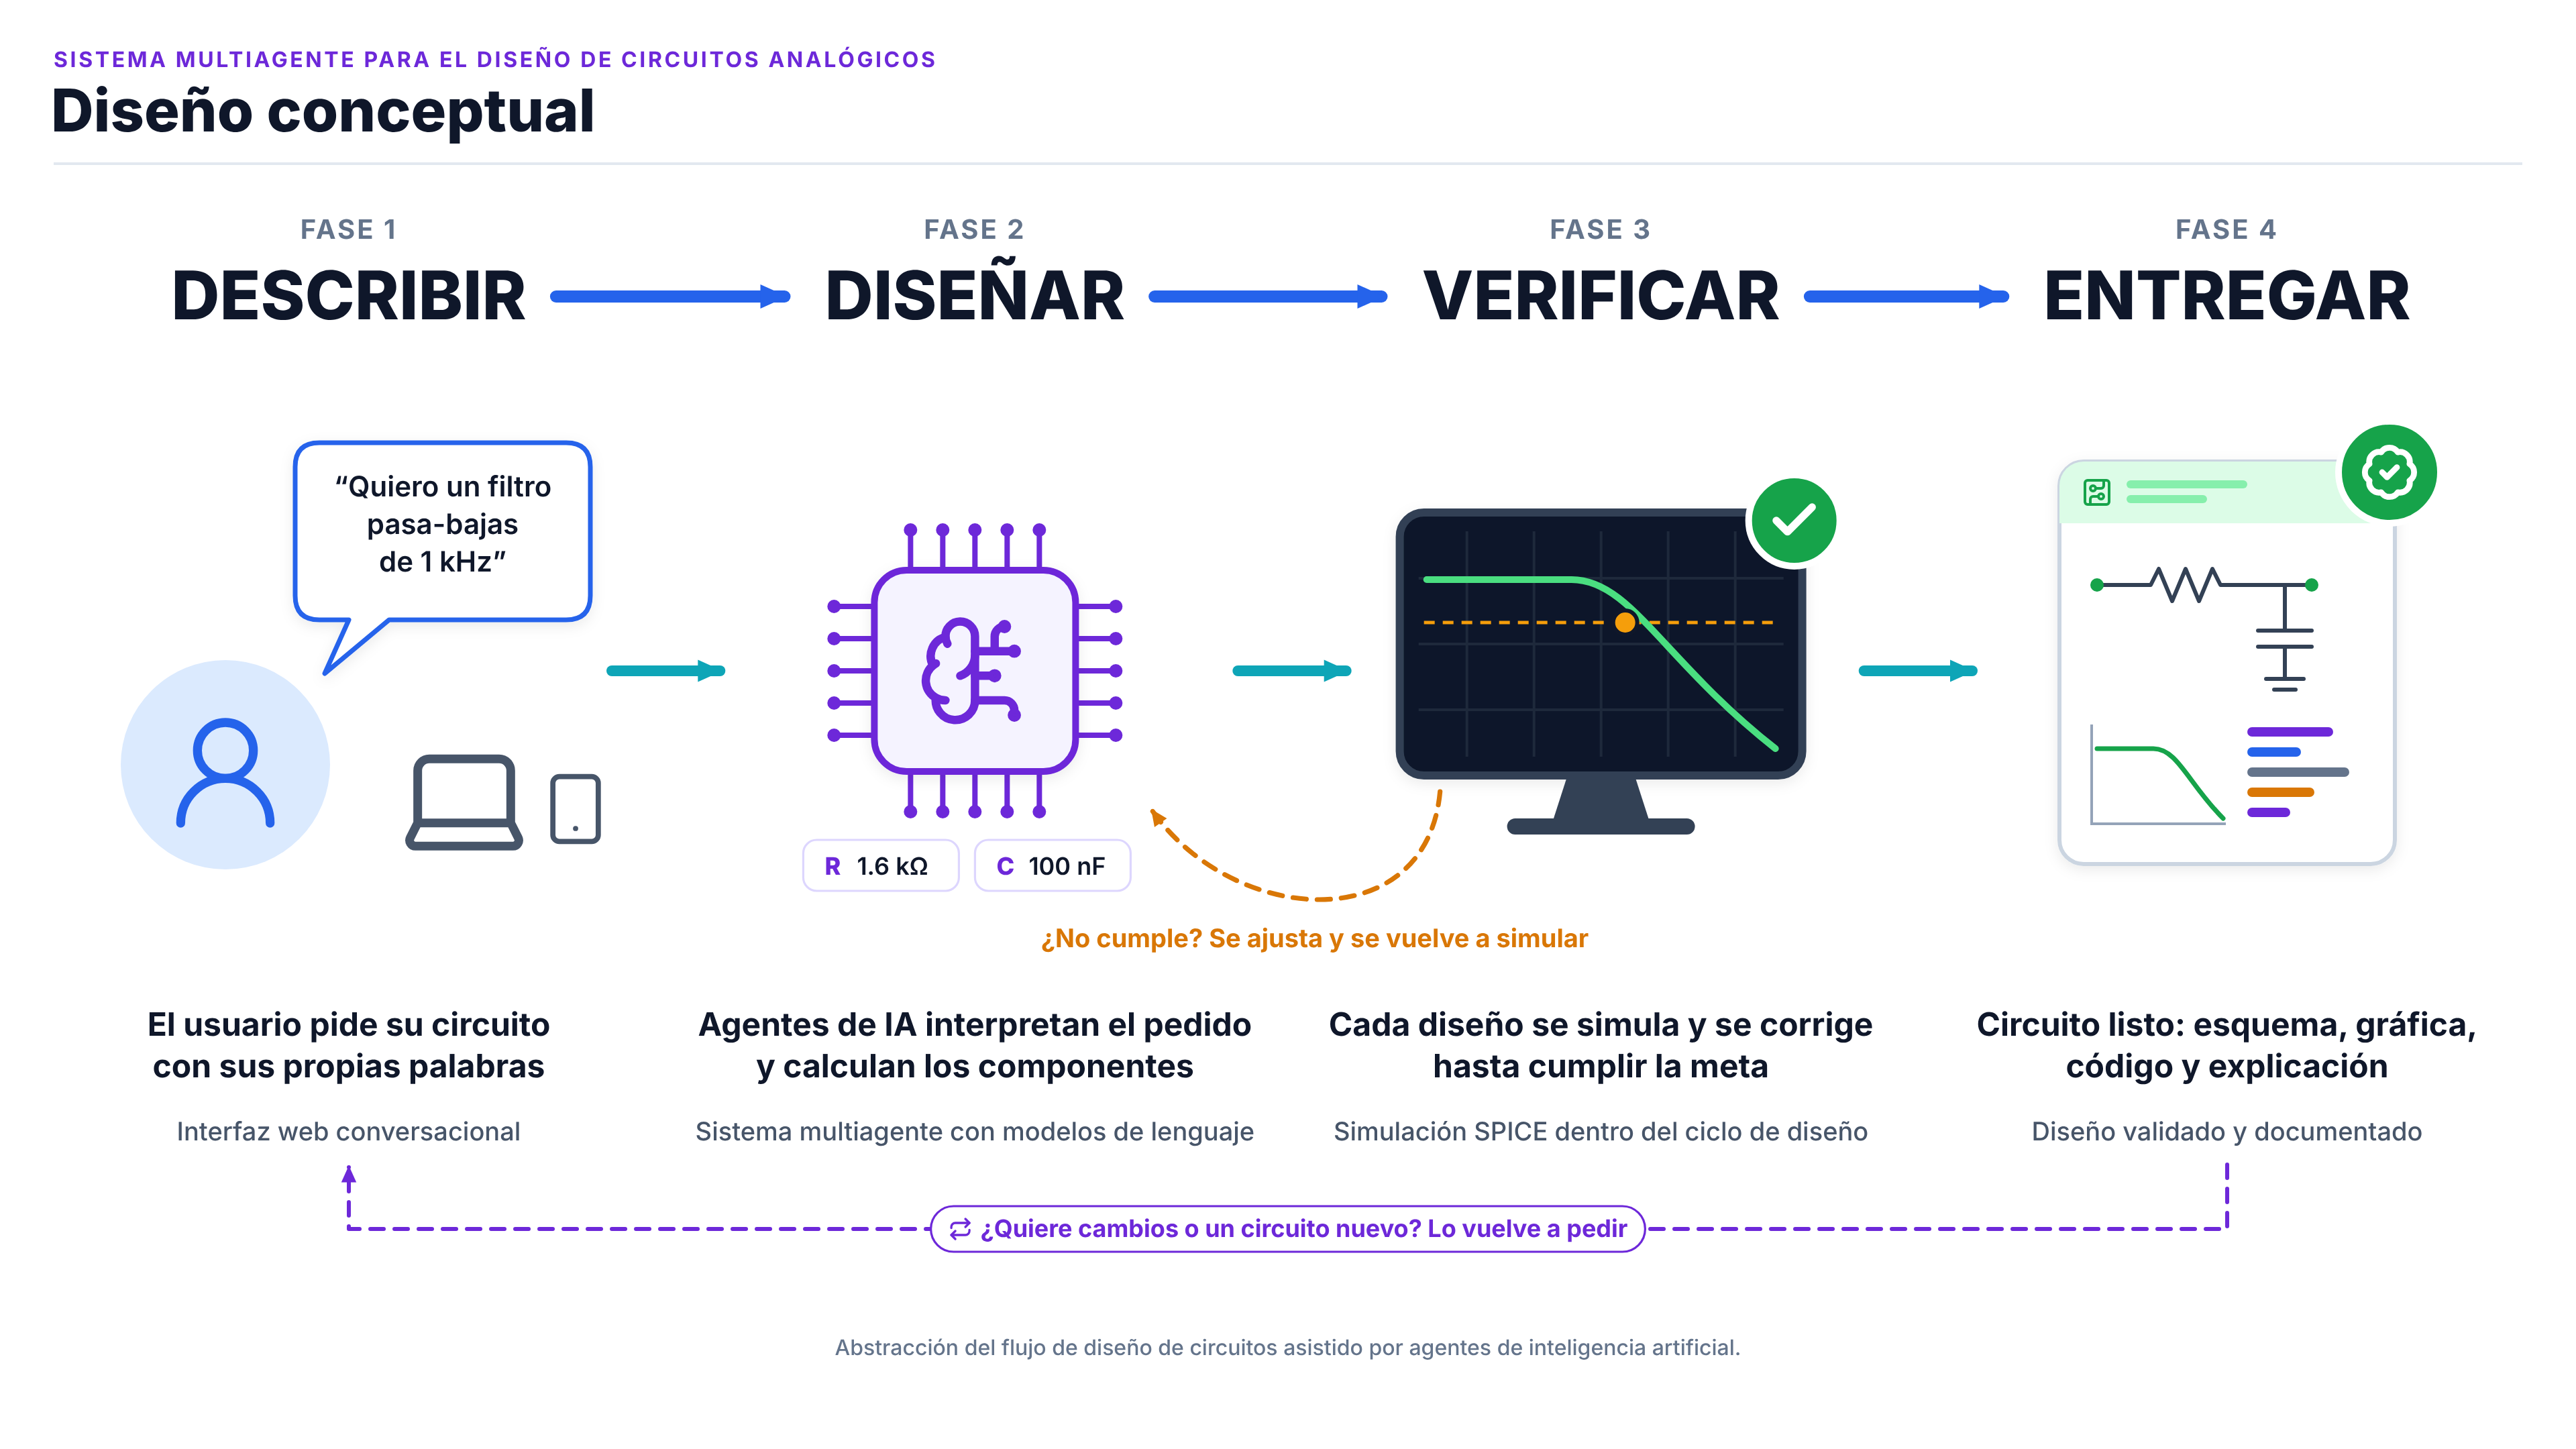
\includegraphics[width=1.2\textwidth, keepaspectratio]{../src/diagrams/diseno_conceptual_fases.png}%
    }
    \caption{Diseño conceptual del sistema en cuatro fases: describir, diseñar, verificar y entregar.}
    \label{fig:diseno-conceptual-fases}
\end{figure}

\section{Descomposición funcional y casos de uso}
\label{sec:prop-funcional}

\subsection{Vista funcional}
\label{subsec:prop-vista-funcional}

Las tareas principales que realiza el sistema se resumen en tres requerimientos funcionales fundamentales (el listado completo se incluye en los anexos):

\begin{itemize}
    \item \textbf{RF-01 Interpretación de la solicitud:} Recibir la descripción del usuario en lenguaje natural, identificar los parámetros eléctricos y elegir la ruta correspondiente: responder una consulta general, pedir algún dato faltante, analizar un circuito dado o diseñar un circuito nuevo.
    \item \textbf{RF-02 Cálculo y armado del circuito con valores definidos:} Dividir el diseño en bloques cuando consta de varias etapas, calcular en paralelo el valor de sus componentes, ajustarlos a series de valores definidos y generar el archivo SPICE listo para simular.
    \item \textbf{RF-03 Simulación en lazo cerrado y entrega de resultados:} Simular el circuito en \texttt{ngspice}, comparar las mediciones contra la meta solicitada para decidir si se acepta o se ajusta el diseño, y entregar al usuario el circuito final junto con su lista de materiales, gráficas y explicación.
\end{itemize}

El diagrama funcional de la figura~\ref{fig:diagrama-funcional} muestra cómo se encadenan estas funciones desde que entra el mensaje del usuario hasta que se obtiene el circuito validado.

% =======================================================================
% NOTA PARA EL AUTOR — DIAGRAMA POR HACER #1: DIAGRAMA FUNCIONAL (en SVG)
% Ruta sugerida: ../src/diagrams/diagrama_funcional.svg
% =======================================================================
\begin{figure}[H]
    \centering
    \IfFileExists{../src/diagrams/diagrama_funcional.png}{%
        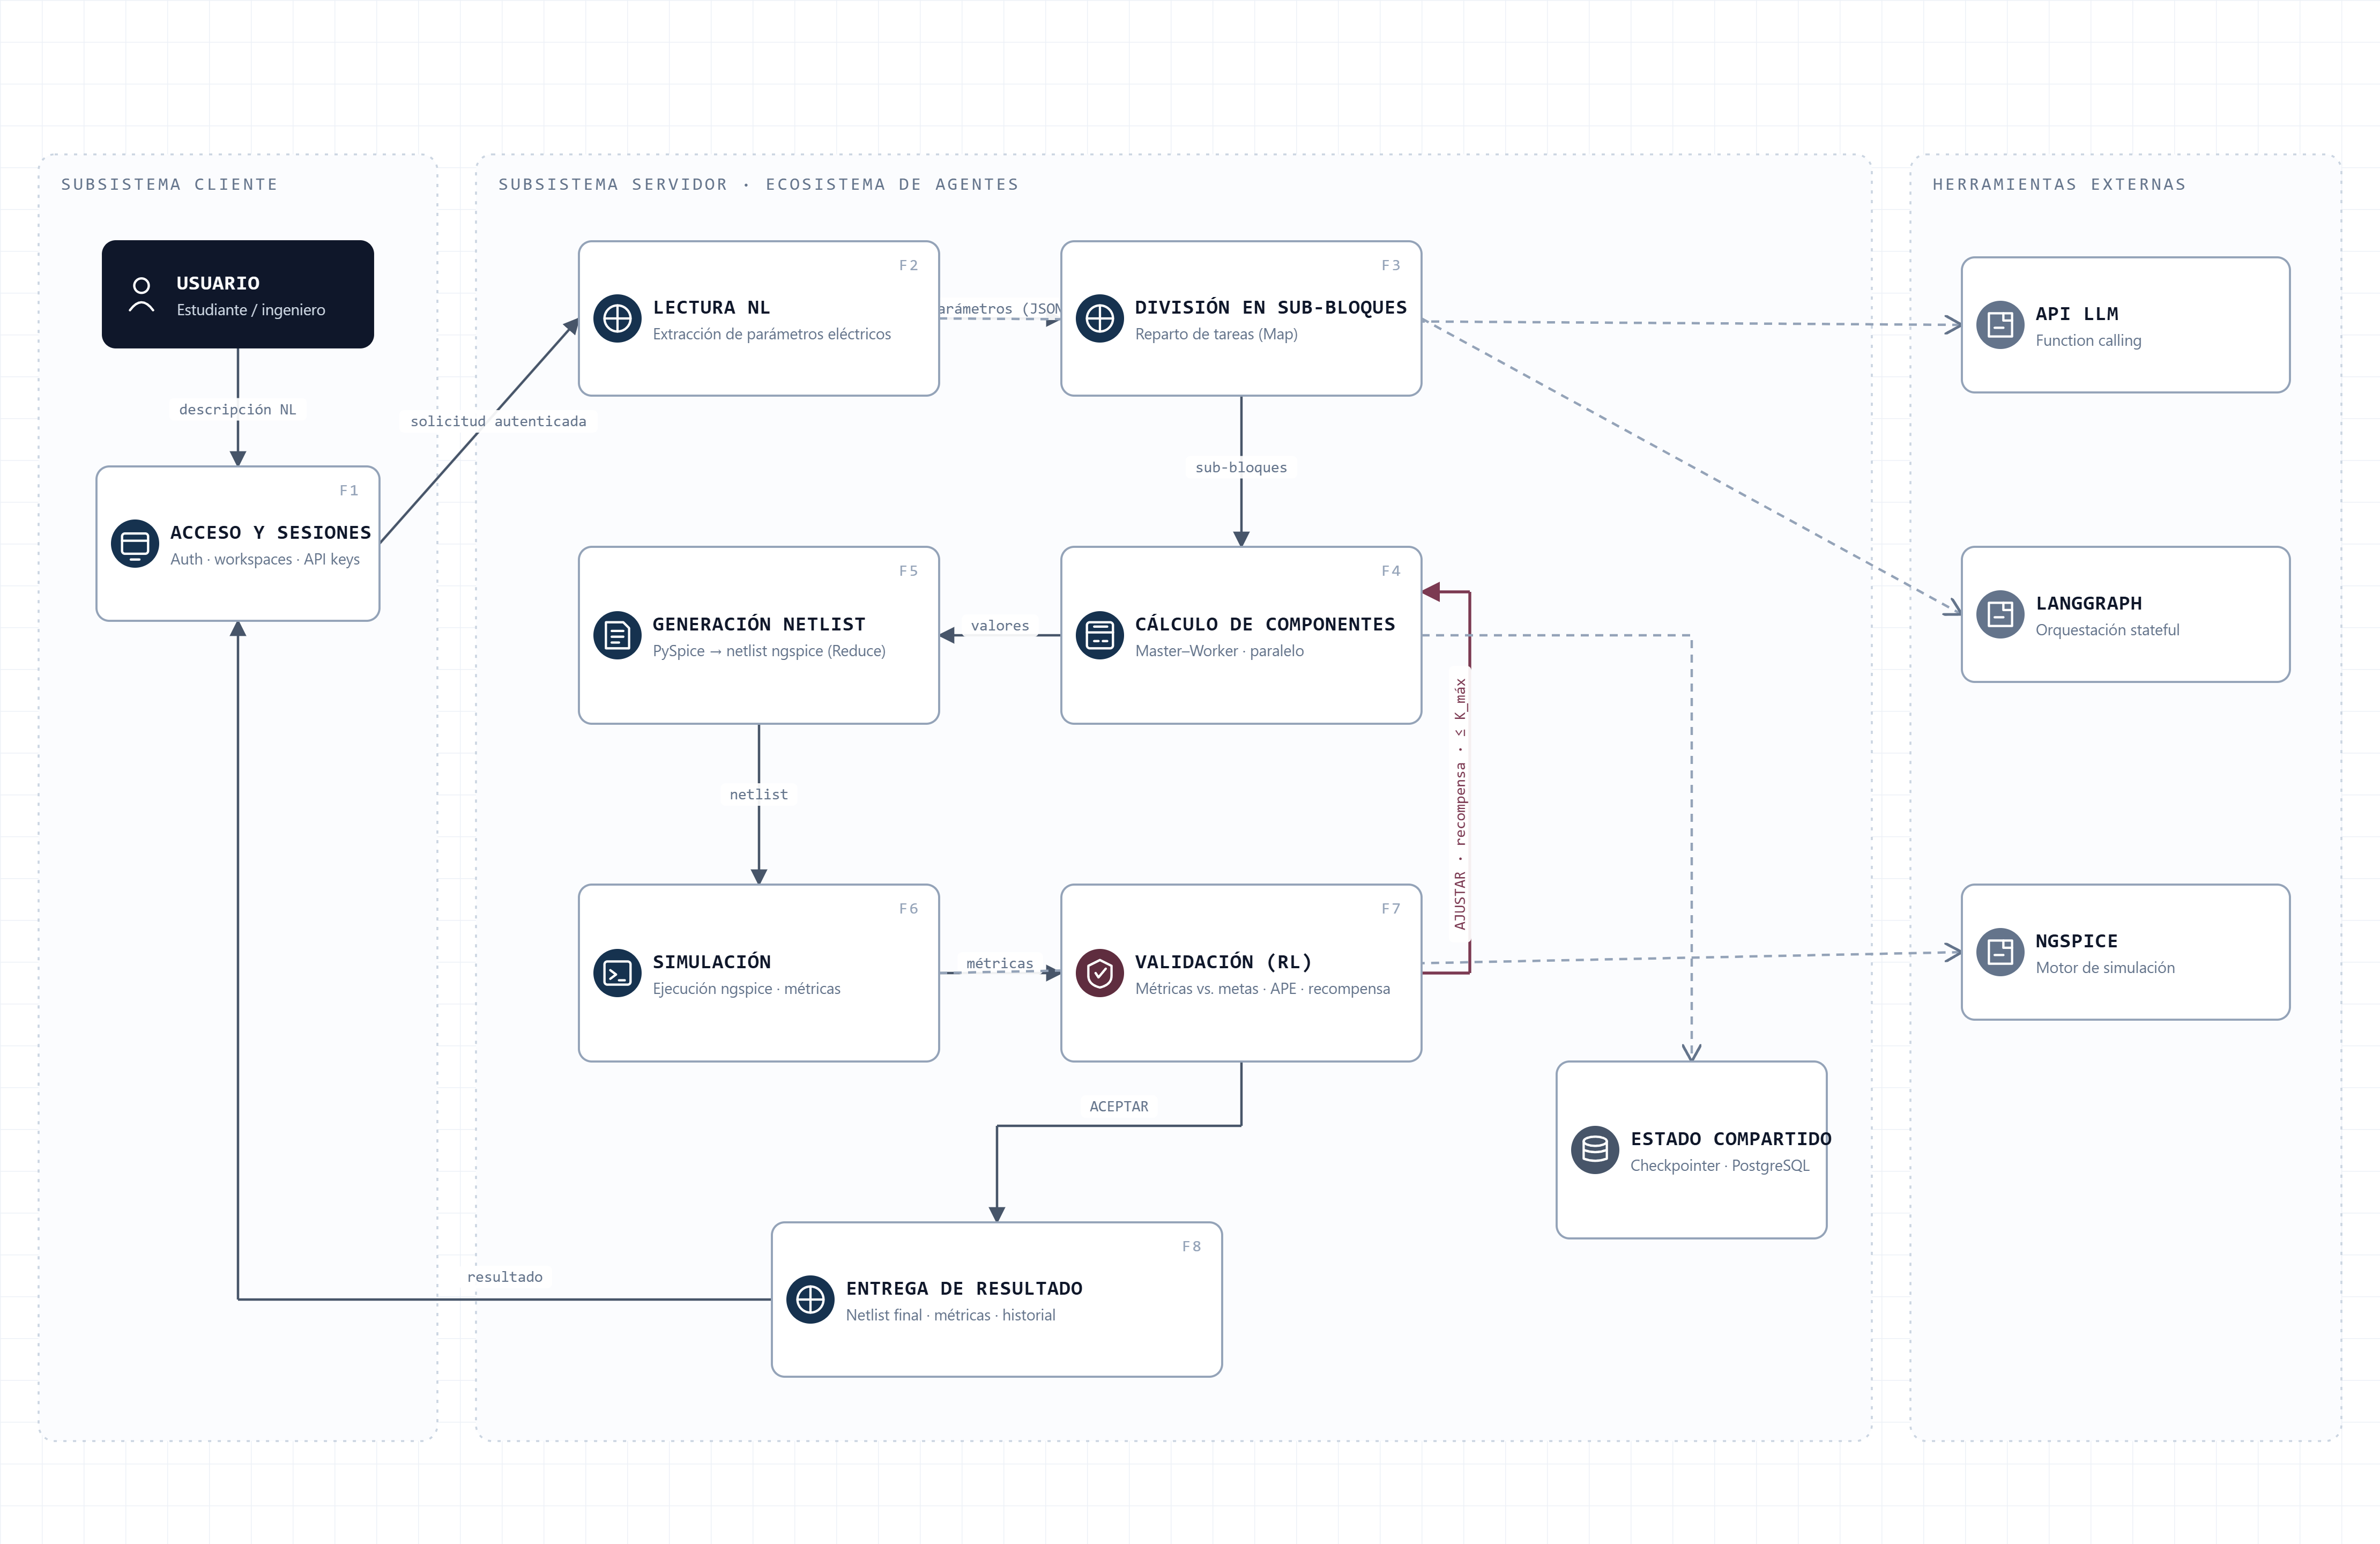
\includegraphics[width=1.0\textwidth, keepaspectratio]{../src/diagrams/diagrama_funcional.png}%
    }{%
        \fbox{\parbox{0.92\textwidth}{\footnotesize\textbf{Diagrama por agregar (SVG):} \texttt{../src/diagrams/diagrama\_funcional.svg}\\[4pt]
        Flujo funcional: Entrada en lenguaje natural $\rightarrow$ Interpretación (Orquestador) $\rightarrow$ Cálculo y ajuste a valores definidos $\rightarrow$ Escritura de netlist $\rightarrow$ Simulación (\texttt{ngspice}) $\rightarrow$ Evaluación (Curador: aceptar, ajustar o rechazar) $\rightarrow$ Entrega documentada.}}%
    }
    \caption{Diagrama funcional del sistema.}
    \label{fig:diagrama-funcional}
\end{figure}

\subsection{Casos de uso}
\label{subsec:prop-casos-uso}

En el sistema intervienen dos tipos de actores: el usuario (estudiante o ingeniero electrónico), que interactúa con la aplicación web, y los servicios externos (el proveedor de modelos de inteligencia artificial y Langfuse), que el sistema consulta durante cada corrida.

Desde la aplicación web, el usuario puede crear su cuenta e iniciar sesión, registrar sus llaves de acceso a proveedores de inteligencia artificial (en la nube o locales) y elegir qué modelo usará cada agente. Asimismo, puede organizar sus conversaciones en proyectos, solicitar el diseño o análisis de un circuito en lenguaje natural y revisar los resultados en el visualizador de circuitos. Los diagramas de casos de uso detallados se encuentran en el apéndice~\ref{apend:casos-uso}.

\section{Arquitectura del sistema (modelo C4)}
\label{sec:prop-c4}

La arquitectura se describe mediante el modelo C4 en tres niveles: el contexto general, los contenedores que integran la plataforma y los componentes internos del servicio de agentes.

\subsection{Nivel 1 — Contexto}
\label{subsec:prop-c4-nivel1}

El nivel de contexto ubica al sistema frente al usuario y los servicios externos con los que se comunica. El usuario ingresa desde su navegador para describir el circuito que desea y consultar el resultado validado. Por su parte, el sistema se conecta con el proveedor de inteligencia artificial configurado por el usuario para las tareas de lenguaje y con Langfuse para consultar las instrucciones de cada agente y registrar las trazas de ejecución, como se muestra en la figura~\ref{fig:c4-nivel1}.

% =======================================================================
% NOTA PARA EL AUTOR — DIAGRAMA POR HACER #2: C4 NIVEL 1 CONTEXTO (en SVG)
% Ruta sugerida: ../src/diagrams/c4_l1_contexto.svg
% =======================================================================
\begin{figure}[H]
    \centering
    \IfFileExists{../src/diagrams/c4_l1_contexto.png}{%
        \includegraphics[width=1.0\textwidth, keepaspectratio]{../src/diagrams/c4_l1_contexto.png}%
    }{%
        \fbox{\parbox{0.92\textwidth}{\footnotesize\textbf{Diagrama por agregar (SVG):} \texttt{../src/diagrams/c4\_l1\_contexto.svg}\\[4pt]
        Elementos C4 Nivel 1: Usuario $\leftrightarrow$ Sistema SPICE $\leftrightarrow$ Sistemas externos (Proveedor de IA y Langfuse).}}%
    }
    \caption{C4 Nivel 1: Diagrama de contexto del sistema.}
    \label{fig:c4-nivel1}
\end{figure}

\subsection{Nivel 2 — Contenedores}
\label{subsec:prop-c4-nivel2}

El nivel de contenedores divide la plataforma en cuatro bloques principales que se levantan con Docker Compose: la aplicación web, el servidor de la aplicación, el servicio de agentes y la base de datos.

La \textbf{aplicación web} (desarrollada con React, Vite y TypeScript) ofrece el chat, la organización de proyectos y archivos, la elección del modelo de IA para cada agente y la visualización del esquema, las gráficas y el código SPICE. Se comunica con el servidor mediante HTTP/JSON para pedir y guardar datos, y recibe el avance de cada corrida en vivo por medio de eventos SSE (\textit{Server-Sent Events}).

El \textbf{servidor de la aplicación} (construido con Bun, Hono, Drizzle y Better Auth) gestiona las cuentas y sesiones, los proyectos y conversaciones, las llaves de IA cifradas y el catálogo de circuitos. Se encarga de probar las llaves ante el proveedor de IA, iniciar cada corrida en el servicio de agentes (\texttt{POST /runs}) y reenviar su avance en vivo al navegador.

El \textbf{servicio de agentes} (implementado en Python con LangGraph, FastAPI y PySpice) coordina en un grafo a los seis agentes del sistema —Orquestador, Cálculo, Escritura, Simulación, Curador y Documentador— y ejecuta dentro del mismo contenedor el simulador \texttt{ngspice}. Durante una corrida, consulta al servidor el modelo asignado y el catálogo por una API interna, pide las instrucciones y registra la traza en Langfuse, consulta al proveedor de IA (Anthropic, OpenAI, Gemini, Ollama o LM Studio) y guarda los puntos de control del grafo.

Finalmente, la \textbf{base de datos} (PostgreSQL en Neon) almacena los usuarios, conversaciones, resultados, el catálogo de circuitos, las llaves cifradas y los puntos de control. La relación entre los cuatro contenedores y los sistemas externos se ilustra en la figura~\ref{fig:c4-nivel2}.

\begin{figure}[H]
    \centering
    \makebox[\textwidth][c]{%
        \hspace*{-0.5cm}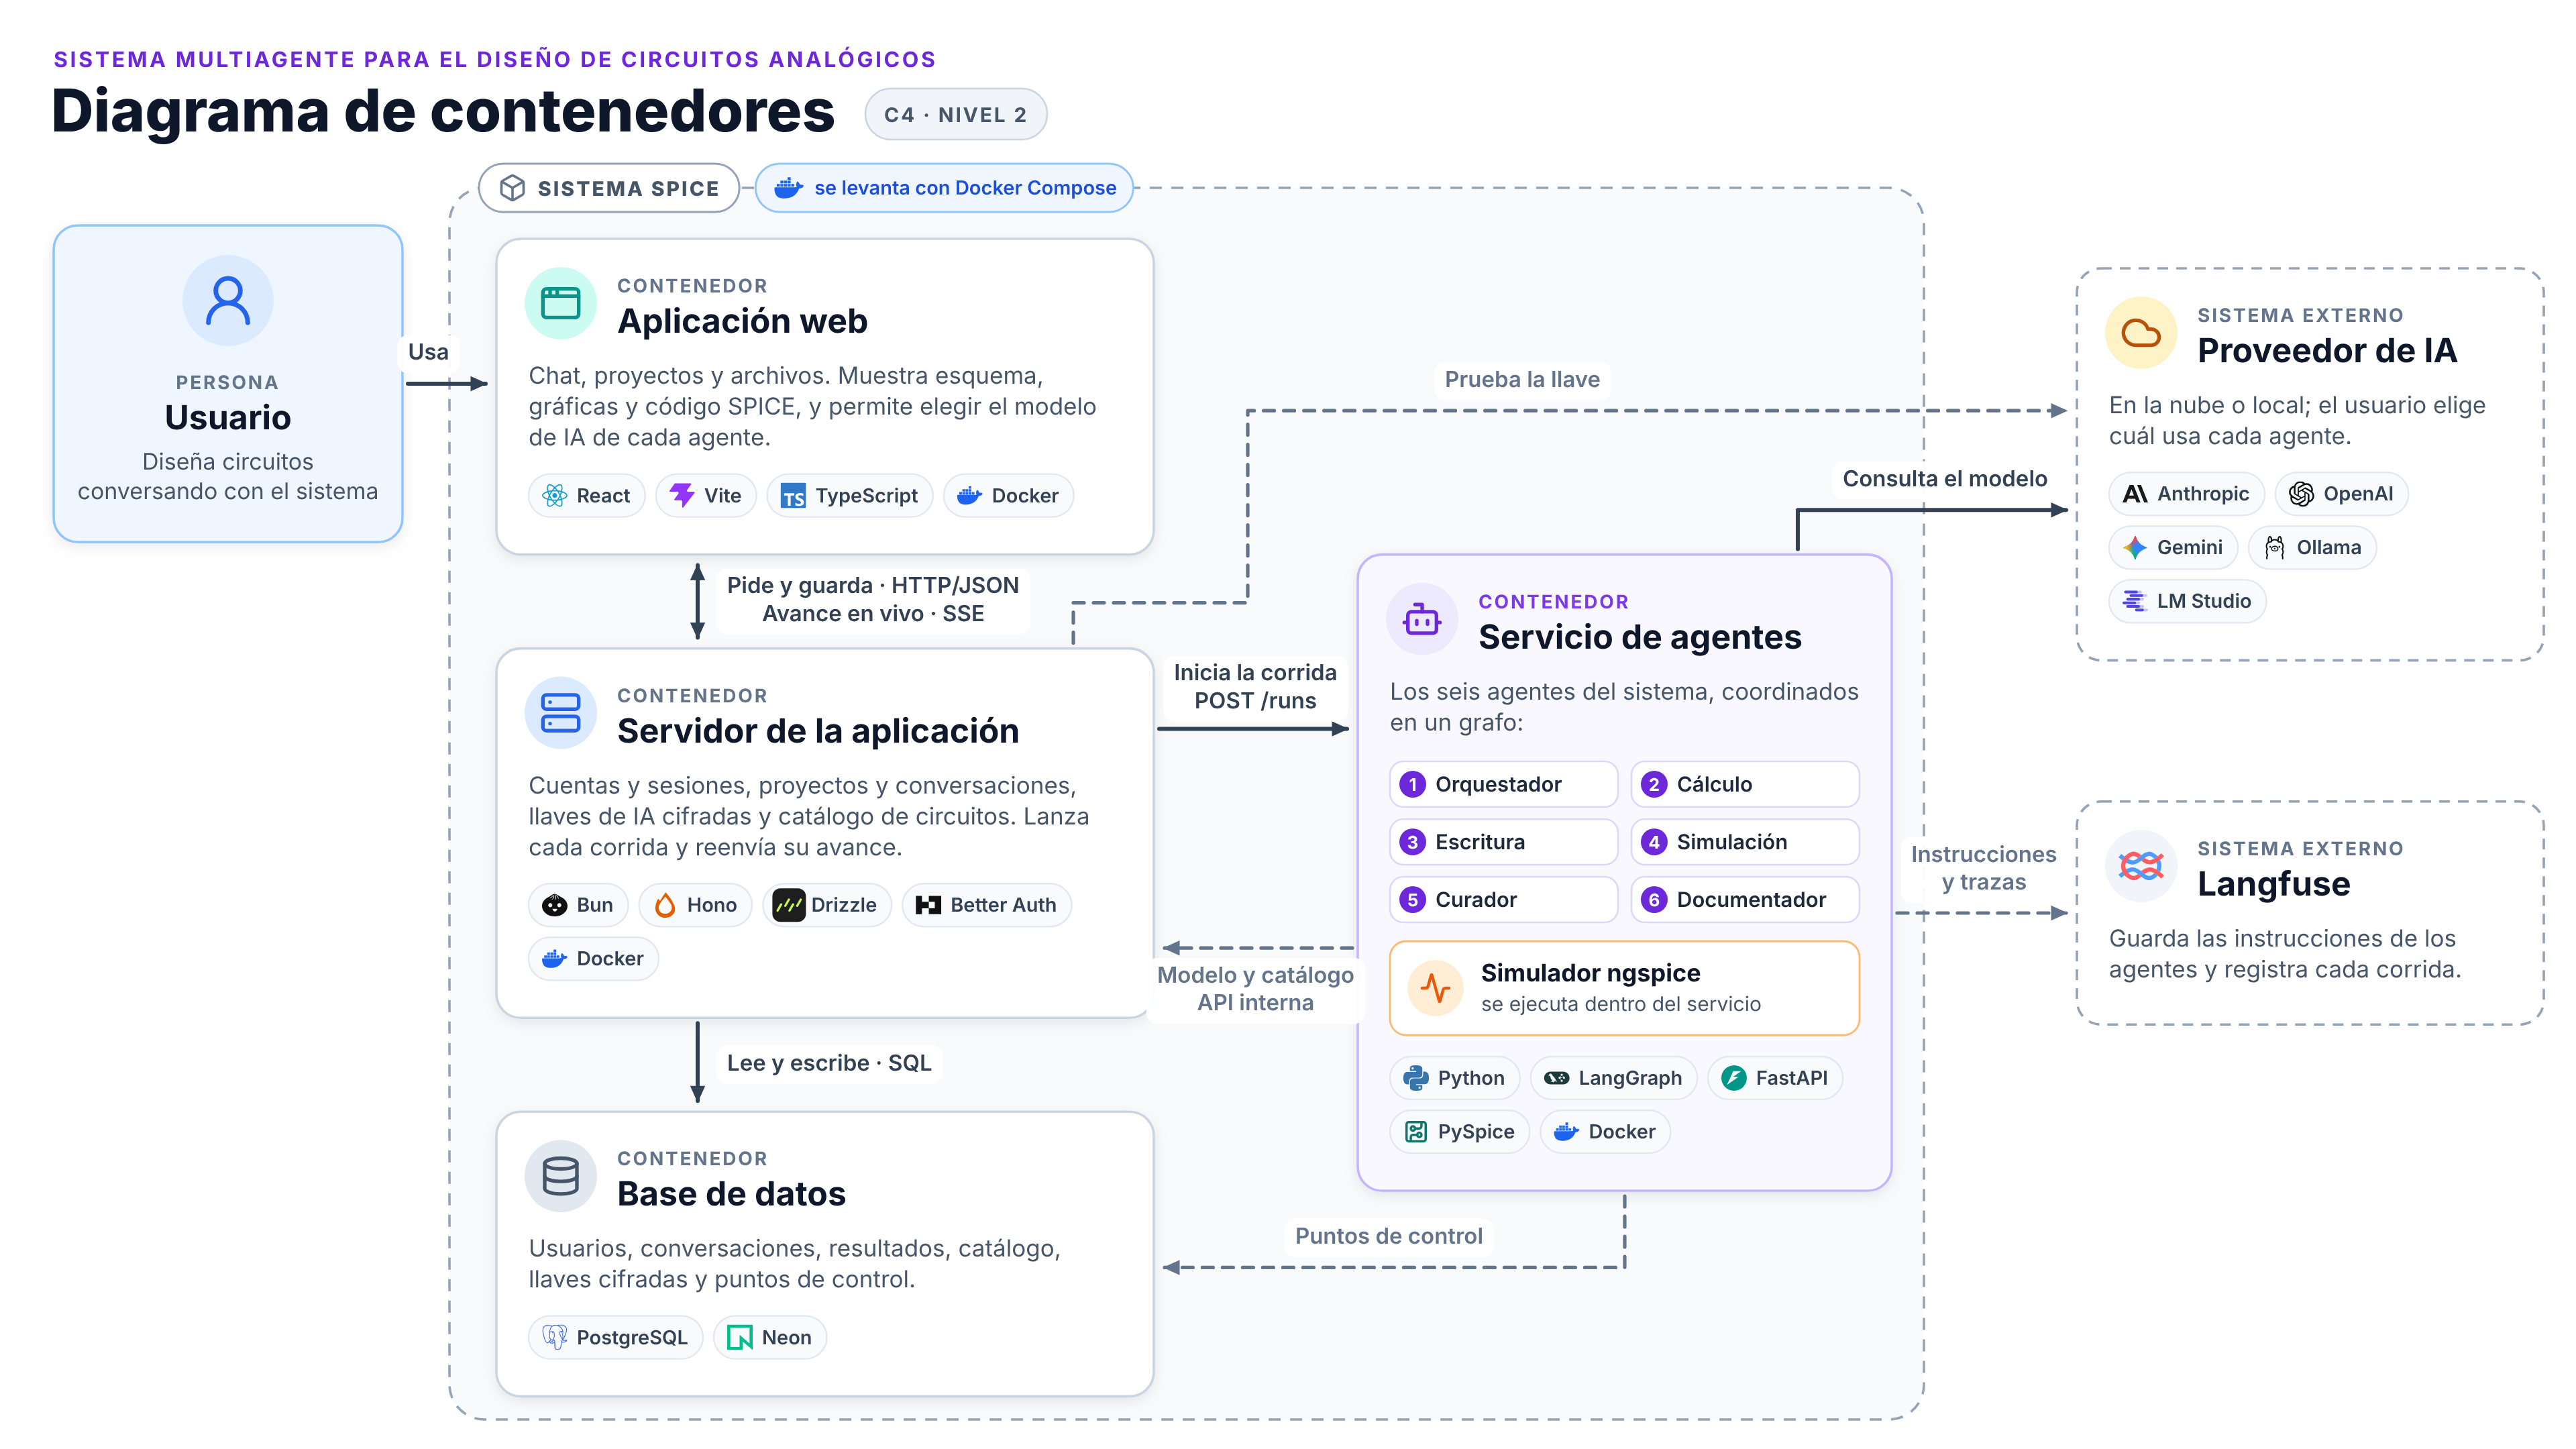
\includegraphics[width=1.2\textwidth, keepaspectratio]{../src/diagrams/C2 - lvl 2.png}%
    }
    \caption{C4 Nivel 2: Diagrama de contenedores del sistema.}
    \label{fig:c4-nivel2}
\end{figure}

\subsection{Nivel 3 — Componentes del servicio de agentes}
\label{subsec:prop-c4-nivel3}

Dentro del servicio de agentes, los componentes se agrupan en tres zonas: coordinación, construcción y validación. En la \textbf{zona de coordinación} se ubica el Orquestador, que recibe el pedido del usuario, consulta el catálogo de circuitos y define qué camino tomar (conversación, aclaración, análisis o diseño), acompañado por el nodo de Análisis —para resolver circuitos ya dados por el usuario— y el guardado de puntos de control.

En la \textbf{zona de construcción} se calculan los componentes, se ajustan a valores definidos y se redacta el archivo SPICE. Para el cálculo de circuitos de una o varias etapas se utiliza un esquema Maestro-Trabajador (\textit{Master/Worker}) en paralelo: el Maestro de Cálculo recibe la especificación del Orquestador y crea un Trabajador independiente por cada sub-bloque del circuito. Cada Trabajador revisa su bloque: si pertenece al catálogo, calcula sus componentes con la fórmula correspondiente; y si es un bloque genérico, pasa tal cual el circuito propuesto por el modelo de lenguaje. Cuando todos los Trabajadores terminan, una barrera reúne los valores en el estado del circuito para avanzar a la etapa de Síntesis, como se muestra en la figura~\ref{fig:calculo-master-worker}.

\begin{figure}[H]
    \centering
    \makebox[\textwidth][c]{%
        \hspace*{-0.5cm}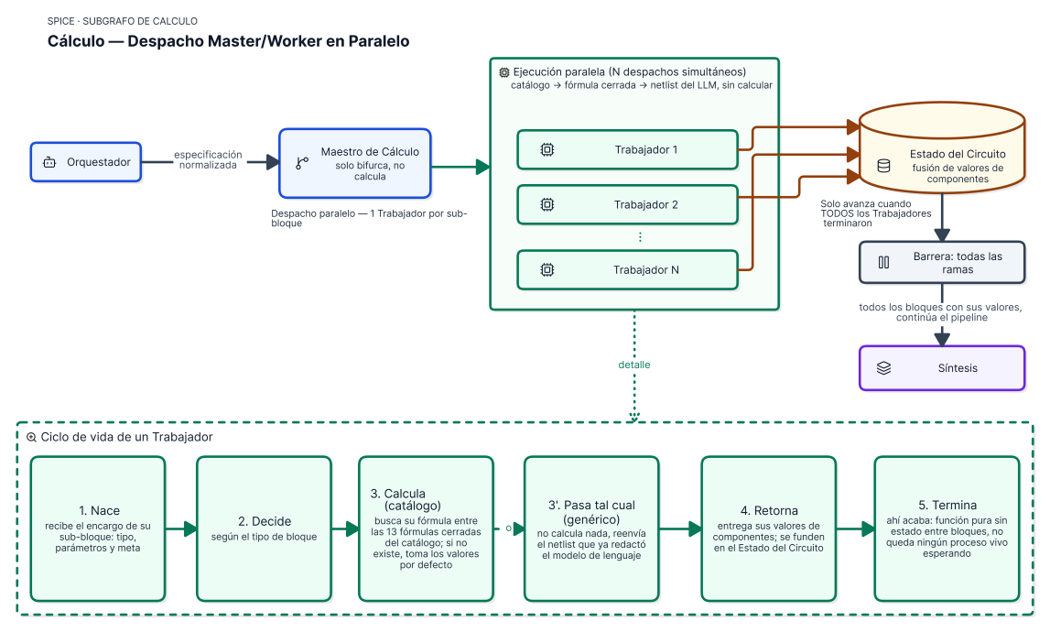
\includegraphics[width=1.2\textwidth, keepaspectratio]{../src/diagrams/Diagrama Master worker en paralelo.png}%
    }
    \caption{Subgrafo de Cálculo: despacho Maestro-Trabajador en paralelo y ciclo de vida de cada trabajador.}
    \label{fig:calculo-master-worker}
\end{figure}

Una vez reunidos los valores ideales, se ajustan las resistencias, capacitores e inductores a valores definidos de series estándar junto con modelos definidos de semiconductores, y el agente de Escritura arma la lista de materiales y el archivo \texttt{.cir}.

Por último, en la \textbf{zona de validación y entrega}, el agente de Simulación corre el archivo en \texttt{ngspice} para leer las métricas y gráficas de respuesta, el Curador evalúa si se cumple la meta del usuario o si hace falta ajustar valores, y el Documentador genera la explicación final del diseño. La integración de estas tres zonas se presenta en la figura~\ref{fig:c4-nivel3}.

% =======================================================================
% NOTA PARA EL AUTOR — DIAGRAMA POR HACER #3: C4 NIVEL 3 COMPONENTES (en SVG)
% Ruta sugerida: ../src/diagrams/c4_l3_agentes.svg
% =======================================================================
\begin{figure}[H]
    \centering
    \IfFileExists{../src/diagrams/c4_l3_agentes.png}{%
        \includegraphics[width=1.0\textwidth, keepaspectratio]{../src/diagrams/c4_l3_agentes.png}%
    }{%
        \fbox{\parbox{0.92\textwidth}{\footnotesize\textbf{Diagrama por agregar (SVG):} \texttt{../src/diagrams/c4\_l3\_agentes.svg}\\[4pt]
        Elementos C4 Nivel 3 (3 zonas): 1.~Coordinación (Orquestador, Análisis y puntos de control); 2.~Construcción (Maestro de Cálculo, Trabajadores en paralelo, ajuste a valores definidos y Escritura); 3.~Validación y entrega (Simulación \texttt{ngspice}, Curador y Documentador).}}%
    }
    \caption{C4 Nivel 3: Componentes del servicio de agentes.}
    \label{fig:c4-nivel3}
\end{figure}

\section{Comportamiento dinámico: flujo de generación y validación}
\label{sec:prop-dinamico}

\subsection{Máquina de estados y secuencia de comunicación}
\label{subsec:prop-automata}

El control de flujo entre los agentes se rige por una máquina de estados finita que parte del estado inicial $q_0$ (Orquestador) y contempla tres caminos principales: diseño, análisis y conversación. Cuando el mensaje del usuario es una pregunta conceptual, requiere pedir datos faltantes o resulta inválido, el Orquestador responde y pasa directamente al estado final $F$. Cuando el usuario pide analizar un circuito existente, el flujo pasa al estado $q_A$ (Análisis), donde se resuelve la red y se entrega el informe en $F$ (o vuelve a $q_0$ si requiere corregir algún dato).

Si la solicitud es diseñar un circuito nuevo, el flujo avanza de $q_0$ a $q_1$ (Cálculo) para obtener los valores de cada bloque y enseguida a $q_2$ (Síntesis) para escribir el netlist y simularlo en \texttt{ngspice}. Con las métricas medidas se pasa a $q_3$ (Curador): si hace falta corregir el resultado, regresa a $q_2$ para ajustar y repetir la simulación; y una vez que emite su veredicto (aceptado o rechazado), avanza a $q_4$ (Documentador) para redactar la explicación final y terminar en $F$, tal como se ilustra en la figura~\ref{fig:automata-estados}.

\begin{figure}[H]
    \centering
    \makebox[\textwidth][c]{%
        \hspace*{-0.5cm}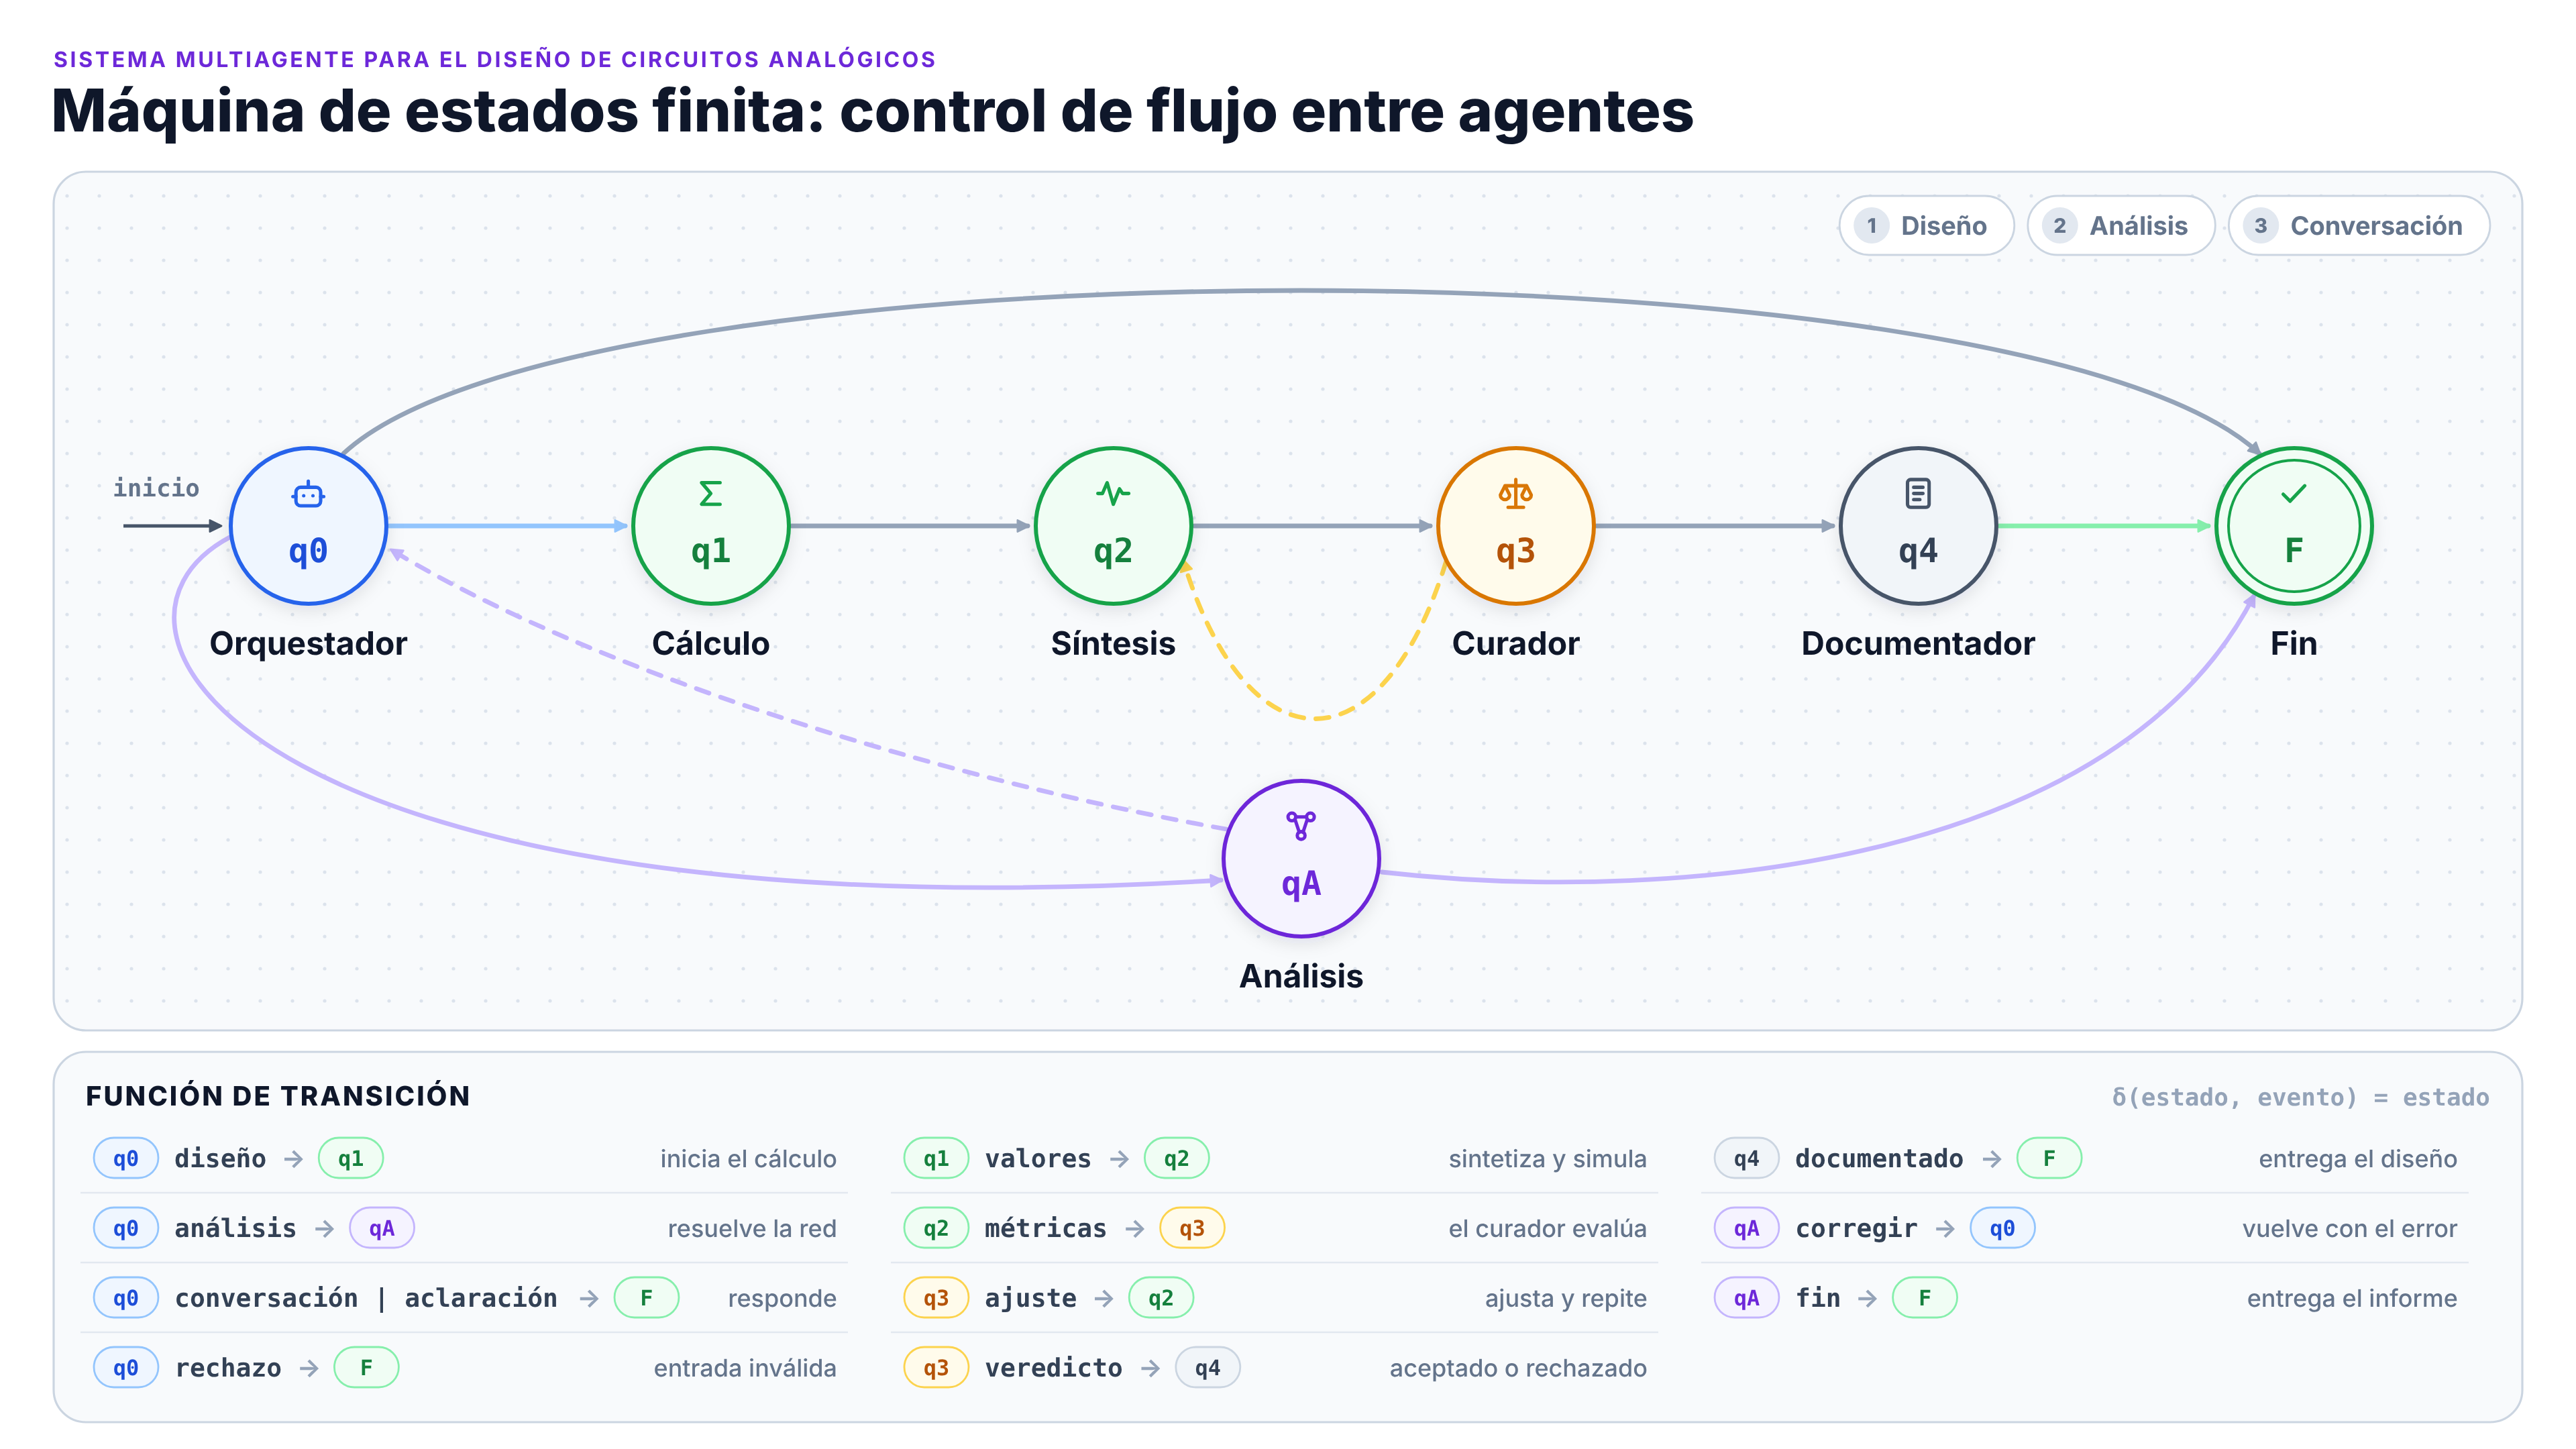
\includegraphics[width=1.2\textwidth, keepaspectratio]{../src/diagrams/automata_estados.png}%
    }
    \caption{Máquina de estados finita y función de transición para el control de flujo entre agentes.}
    \label{fig:automata-estados}
\end{figure}

En el tiempo, este recorrido se inicia cuando el usuario envía su solicitud desde la aplicación web al servidor, el cual delega la corrida al servicio de agentes y retransmite al navegador cada cambio de estado hasta entregar el circuito final, como se muestra en el diagrama de secuencia de la figura~\ref{fig:secuencia-generacion}.

% =======================================================================
% NOTA PARA EL AUTOR — DIAGRAMA POR HACER #4: SECUENCIA (en SVG)
% Ruta sugerida: ../src/diagrams/secuencia_flujo_principal.svg
% =======================================================================
\begin{figure}[H]
    \centering
    \IfFileExists{../src/diagrams/secuencia_flujo_principal.png}{%
        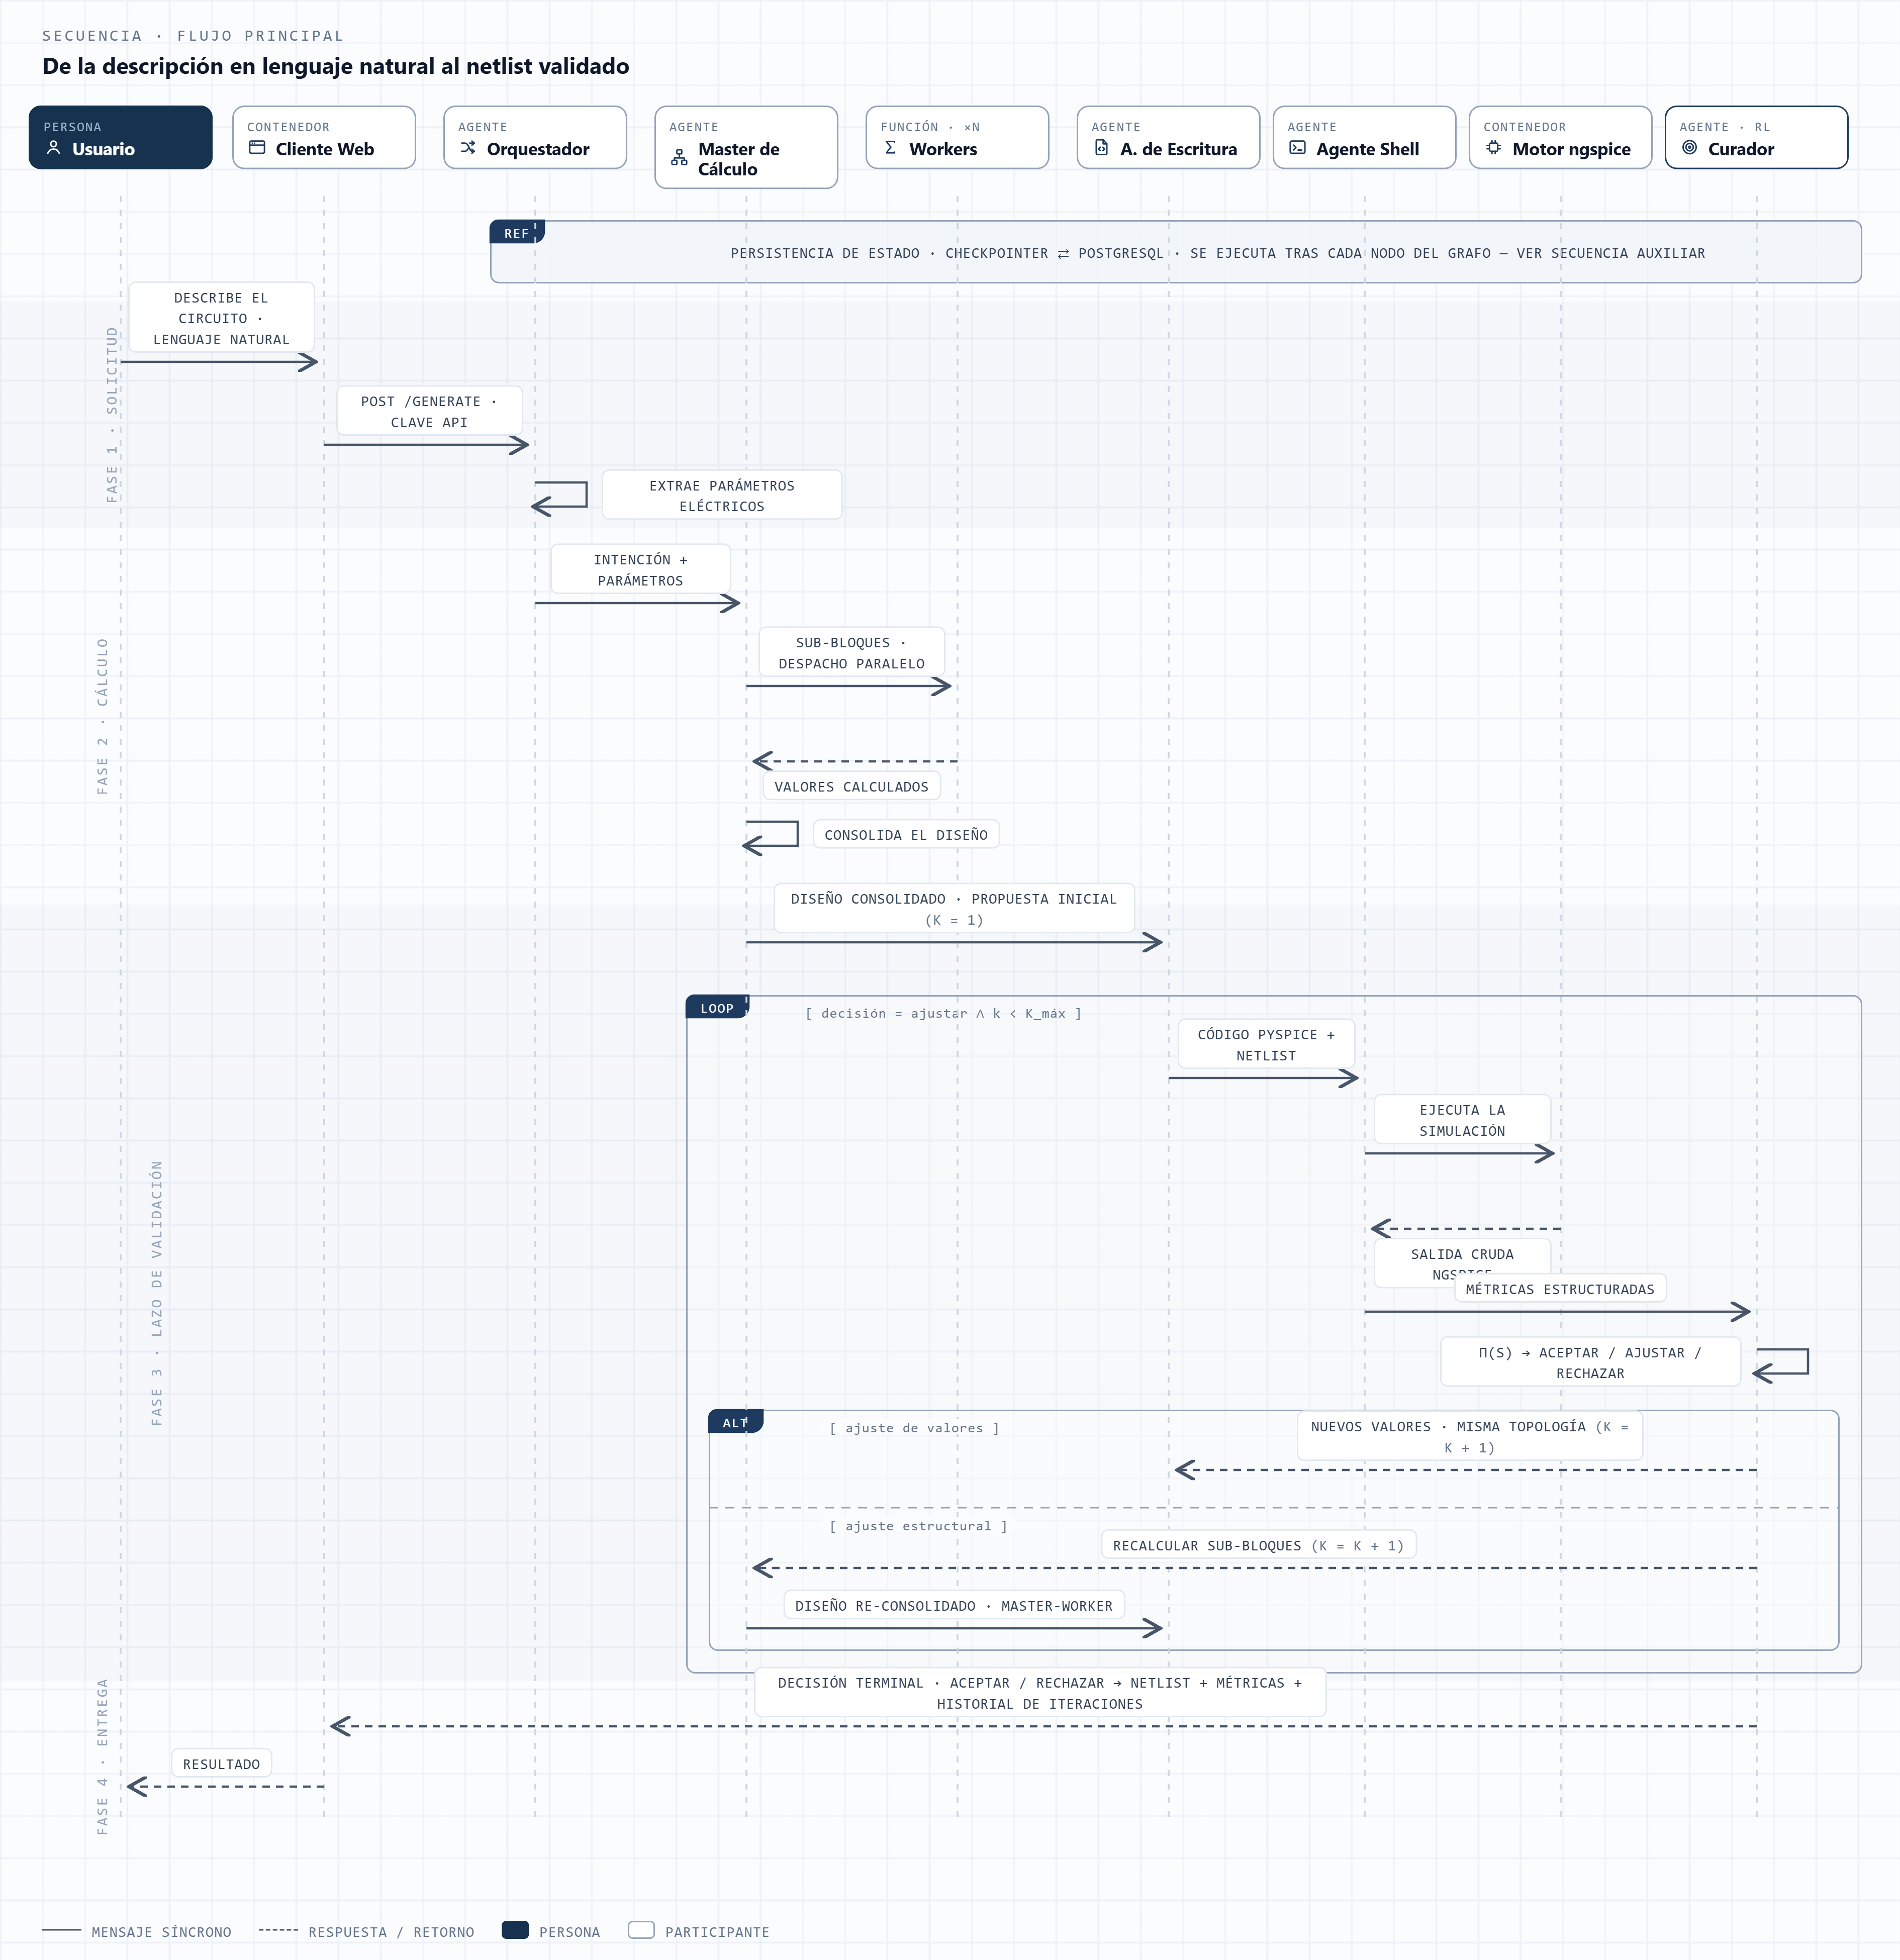
\includegraphics[width=1.0\textwidth, keepaspectratio]{../src/diagrams/secuencia_flujo_principal.png}%
    }{%
        \fbox{\parbox{0.92\textwidth}{\footnotesize\textbf{Diagrama por agregar (SVG):} \texttt{../src/diagrams/secuencia\_flujo\_principal.svg}\\[4pt]
        Secuencia temporal: Usuario $\rightarrow$ Aplicación web $\rightarrow$ Servidor de la aplicación $\rightarrow$ Servicio de agentes (Orquestador $\rightarrow$ Cálculo $\rightarrow$ Lazo [Escritura $\rightarrow$ Simulación \texttt{ngspice} $\rightarrow$ Curador] $\rightarrow$ Documentador) $\rightarrow$ Servidor $\rightarrow$ Aplicación web.}}%
    }
    \caption{Diagrama de secuencia del flujo principal de generación y validación.}
    \label{fig:secuencia-generacion}
\end{figure}

\subsection{Lazo de validación del agente Curador}
\label{subsec:prop-curador-rl}

El ciclo entre la simulación y el agente Curador asegura que el circuito cumpla en la práctica con lo solicitado. Al cambiar los valores calculados por valores definidos, la respuesta simulada en \texttt{ngspice} puede presentar una diferencia frente a la meta ideal. Por ello, en cada intento $n$, el Curador compara el valor medido contra el esperado, obtiene el porcentaje de error ($\text{APE}_i$) y calcula un puntaje de evaluación:

\begin{equation}
    R = -\sum_{i=1}^{M} w_i \cdot \text{APE}_i + \beta \cdot c - \gamma \cdot n
    \label{eq:recompensa-curador}
\end{equation}

En esta expresión, el primer término descuenta el error porcentual de cada meta, el segundo término ($\beta \cdot c$) suma un bono si la simulación en \texttt{ngspice} convergió sin fallos, y el tercer término ($\gamma \cdot n$) resta puntos por cada intento adicional para favorecer soluciones rápidas dentro de una tolerancia del 5\%.

A partir de este resultado, el Curador toma una de tres decisiones: \textbf{aceptar} el diseño cuando el error está dentro de la tolerancia; \textbf{ajustar} el valor de los componentes (o combinar dos piezas en serie o paralelo si un solo valor redondeado no basta) para simular de nuevo; o \textbf{rechazar} la corrida si se alcanza el límite de intentos, entregando en ese caso la iteración que haya tenido el menor error. Este flujo de decisión se muestra en la figura~\ref{fig:curador-flujo}.

\begin{figure}[H]
    \centering
    \makebox[\textwidth][c]{%
        % Preferir versión vectorial SVG: ../src/diagrams/curador_flujo.svg
        \hspace*{-0.5cm}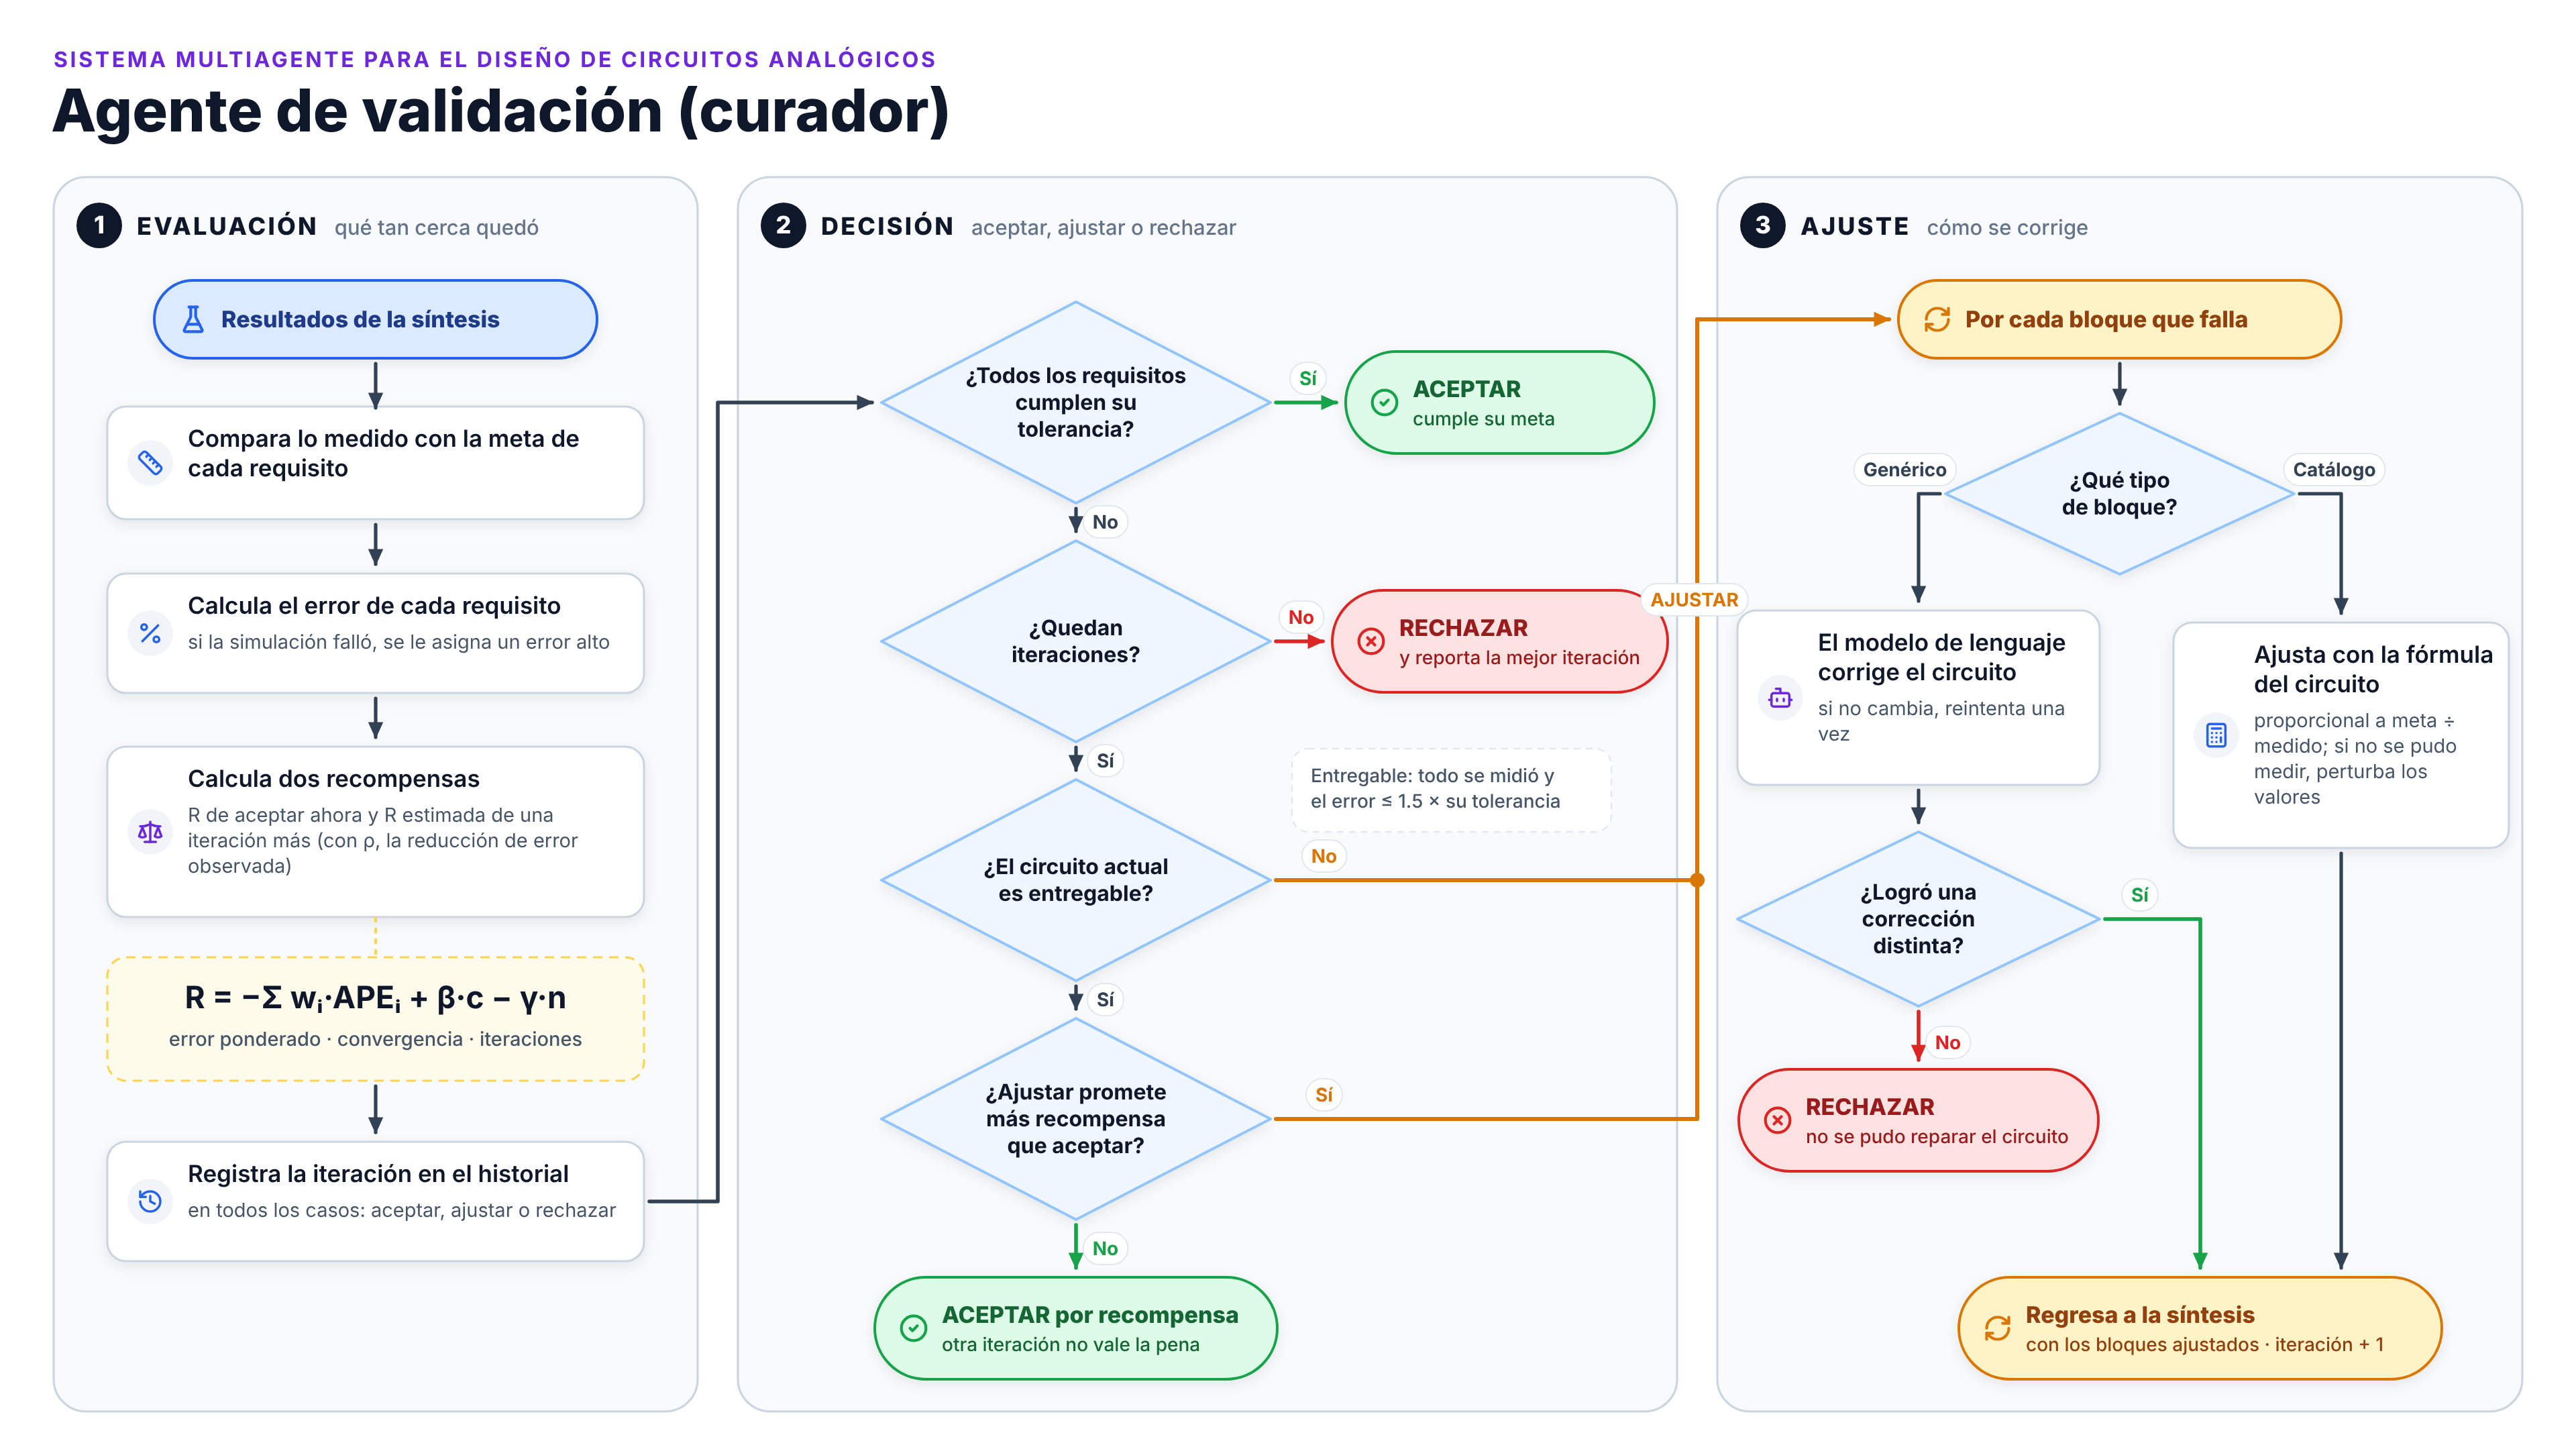
\includegraphics[width=1.2\textwidth, keepaspectratio]{../src/diagrams/curador_flujo.png}%
    }
    \caption{Flujo de evaluación, decisión y ajuste del agente Curador.}
    \label{fig:curador-flujo}
\end{figure}
